\section{Experimentos numéricos}



En esta sección mostraremos soluciones obtenidas numéricamente del problema de control presentado. 
%
Para ello primero explicaremos como la metodología que utilizamos para resolver los problemas de control (\ref{OCP1}) y (\ref{OCP_bn}), y luego mostraremos casos concretos mostrando la precisión obenida y algunos ejemplos donde el número de ángulos varía con respecto al valor de los coeficientes de Fourier considerados.

\subsection{Numerical solution of OCP-SHE}

To solve the optimal control problem (\ref{OCP1}), we use a direct method. 
If we consider a partition $\mathcal{P} = \{\tau_0,\tau_1,\dots,\tau_{T}\}$ of interval $[0,T]$ , we can represent a function $\{ f(\tau) \ | \ \tau \in [0,T]\}$ as a vector $\bm{f} \in \mathbb{R}^{T}$ where component $f_t = f(\tau_t)$. Then the optimal control problem (\ref{OCP1}) can be written as optimization problem with variable $\bm{f} \in \mathbb{R}^{T}$. This problem is a nonlinear programming, for this we use CasADi software to solve. Entonces, dado una partición del intervalo $[0,\pi]$ podemos reformular el problema (\ref{OCP1}) como el siguiente problema en tiempo discreto:

\begin{problem}[OCP numérico con simetría de media onda]
    Dados dos conjuntos de números impares $\mathcal{E}_a$ and $\mathcal{E}_b$ con cardinalidades $|\mathcal{E}_a| = N_a$ y  $|\mathcal{E}_b| = N_b$ respectivamente , dados los vectores objetivos $\bm{a}_T  \in \mathbb{R}^{N_a}$ y $\bm{b}_T  \in \mathbb{R}^{N_b}$ y una  partition $\mathcal{P} = \{\tau_0,\tau_1,\dots,\tau_{T}\}$ of interval $[0,\pi]$. We search a vector $\bm{f} \in \mathbb{R}^{T}$ that minimize the following function:
    \begin{gather}
        \min_{\bm{f} \in \mathbb{R}^{T} } 
        \Bigg[ 
        || \bm{a}_T - \bm{\alpha}^{T}||^2 + 
        || \bm{b}_T - \bm{\beta}^{T}||^2 
        + \epsilon  \sum_{t=0}^{T-1} \mathcal{L}(f_{t}) \Delta\tau_t  \Bigg]  \\
        \notag \text{suject to: } \\
        \notag i \in \mathcal{E}_a \ \ 
        \begin{cases}
            \alpha_i^{t+1} = \alpha_i^{t} + \Delta \tau_t (2/\pi) \cos(i\tau_t) f_t \\
            \alpha_i^0 = 0
        \end{cases} \\
        \notag j \in \mathcal{E}_b \ \ 
        \begin{cases}
            \beta_j^{t+1} = \beta_j^{t} + \Delta \tau_t (2/\pi) \sin(j\tau_t) f_t \\
            \beta_j^0 = 0
        \end{cases} \\
        \notag |f_t| < 1 \ | \  \Delta \tau_t = \tau_{t+1} - \tau_{t} \ | \ \forall t \in \{1,\dots,T-1\}
    \end{gather}
\end{problem}


En el caso del problema con simetría de cuarto de onda siguiendo la misma linea argumental anterior podemos formular el siguiente problema de optimización:

\begin{problem}[OCP numérico con simetría de cuarto de onda]
    Given  a set of odd numbers $\mathcal{E}_b$ with carinality $|\mathcal{E}_b| = N_b$, given the target vector $\bm{b}_T  \in \mathbb{R}^{N_b}$ and  partition $\mathcal{P} = \{\tau_0,\tau_1,\dots,\tau_{T}\}$ of interval $[0,\pi/2]$. We search a vector $\bm{f} \in \mathbb{R}^{T}$ that minimize the following function:
    \begin{gather}
        \min_{\bm{f} \in \mathbb{R}^{T} } 
        \Bigg[ || \bm{b}_T - \bm{\beta}^{T}||^2 +
         \epsilon  \sum_{t=0}^{T-1} \mathcal{L}(f_{t}) \Delta\tau_t  \Bigg]  \\
        \notag \text{suject to: } \\
        \notag j \in \mathcal{E}_b \ \ 
        \begin{cases}
            \beta_j^{t+1} = \beta_j^{t} + \Delta \tau_t (4/\pi) \sin(j\tau_t) f_t \\
            \beta_j^0 = 0
        \end{cases} \\
        \notag |f_t| < 1 \  | \   \Delta \tau_t = \tau_{t+1} - \tau_{t} \ | \ \forall t \in \{1,\dots,T-1\}
    \end{gather}
\end{problem}

\subsection{Resultados}

Cabe mencionar que todas las simulaciones se han realizado con un ordenador de mesa con $8Gb$ de ram, y el tiempo de ejecución para la búsqueda de soluciones dado un vector objetivo es del orden del segundo. A continuación listaremos cada uno de los resultados numéricos obtenidos:
\begin{enumerate}    


    \item \textbf{OCP con simetría de cuarto de onda}: Consideraremos el problema  con un conjunto de números impares $\mathcal{E}_b = \{1,5\}$ con una discretización del intervalo $[0,\pi/2]$ de $T = 200$. Mostramos las soluciones para los vectores objetivo $b_T^1 = \{(-0.4,-0.3,\dots,0.3,0.4)\}$ manteniendo $b_T^5=0$ para todos los casos. Mostramos las trayectorias óptimas obtenidas en la figura (\ref{ex01}), donde se puede ver una continuidad en las soluciones con respecto a vector objetivo.

    \begin{figure}
        \centering
        \begin{subfigure}[b]{\textwidth}
            \centering
            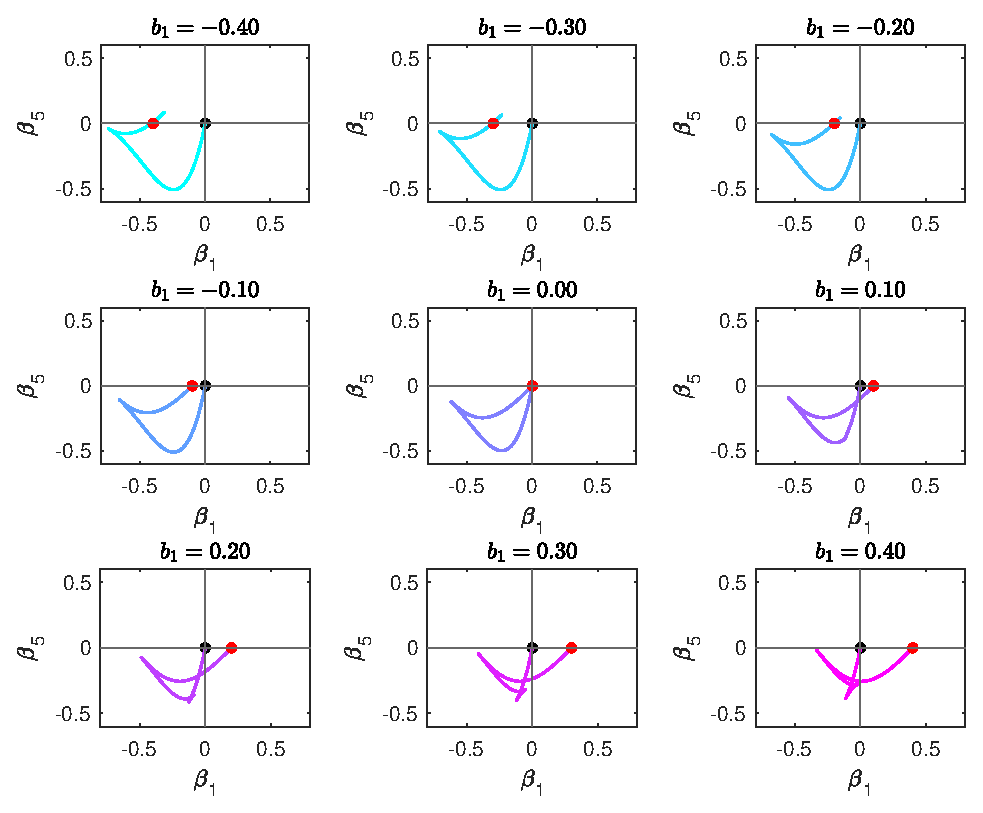
\includegraphics[width=0.6\textwidth]{img/ex01-con.eps}
            \caption{Dynamical System: el punto rojo hace referencia al punto final mientras que el punto negro hace referencia al punto inicial.}
        \end{subfigure} 
        \hfill \\
        \begin{subfigure}[b]{\textwidth}
            \centering
            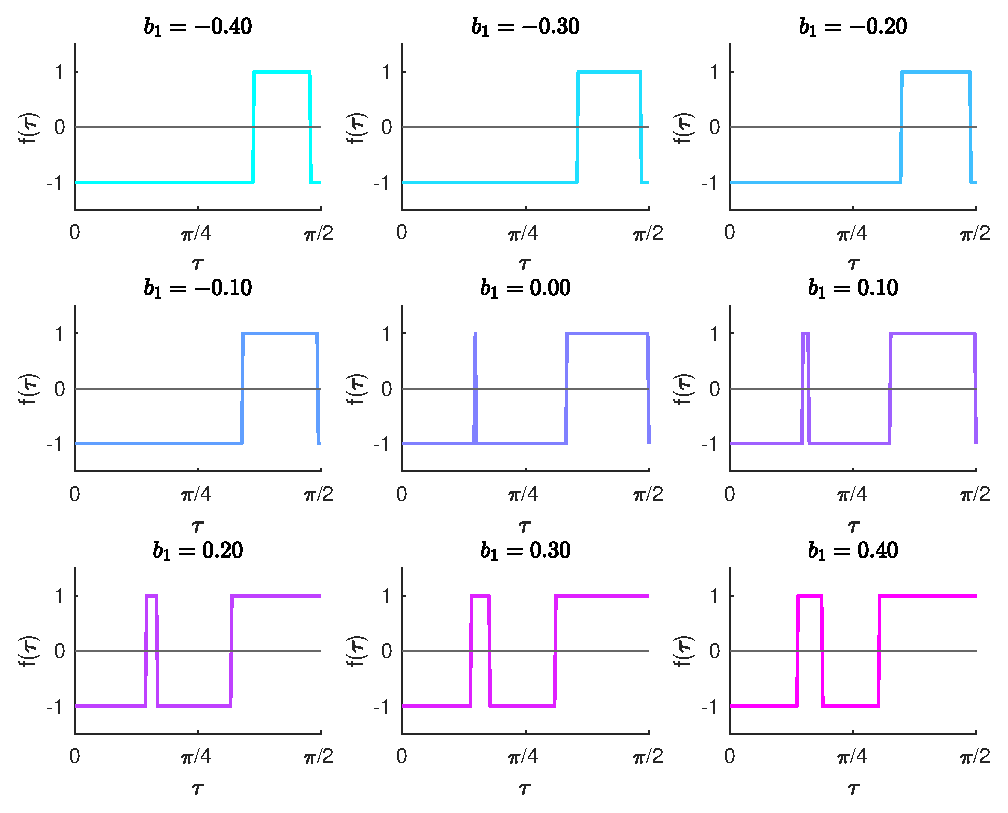
\includegraphics[width=0.6\textwidth]{img/ex01-dyn.eps} 
            \caption{Control}
        \end{subfigure}
        \caption{Mostramos las trayectorias óptimas y controles óptimos para distintos vectores objetivo.}
        \label{ex01}
    \end{figure}


    \item \textbf{OCP con simetría de cuarto onda para un intervalo del $b_1$}: Para este ejemplo consideramos el siguiente conjunto de números impares: $\mathcal{E}_b = \{1,5,7,11,13\}$. 
    %
    Ademas consideramos el vector objetivo $\bm{b}_T = [m_a,0,0,0,0]$, donde  $m_a \in [-1,1]$ es un parámetro. with three penalization terms: $\mathcal{L}(f) = -f$, $\mathcal{L}(f) = +f$ and $\mathcal{L}(f) = -f^2$ obtained by direct method with uniform partition of interval $[0,\pi/2]$ with $T=400$ and penalization parameter $\epsilon = 10^{-5}$. 
    %
    Para cada uno de los términos de penalización utilizados la distancia entre los coeficientes de Fourier se encuentra en el orden de $10^{-4}$. 
    %
    Sin embargo, cuando el término de penalización es $\mathcal{L}(f)= -f^2$ la solución no presenta continudad con respecto al vector objetivo. 
    %
    Por otra parte, es importante mencionar que las soluciones para los términos de penalización $\mathcal{L}(f) = -f$ y $\mathcal{L}(f) = f$ cumplen una simetría por lo que invirtiendo las soluciones con respecto al origen y invirtiendo el signo de las soluciones se puede ver que ambas soluciones son la misma.

    \begin{figure}
        \centering
        \begin{subfigure}[b]{\textwidth}
            \centering
            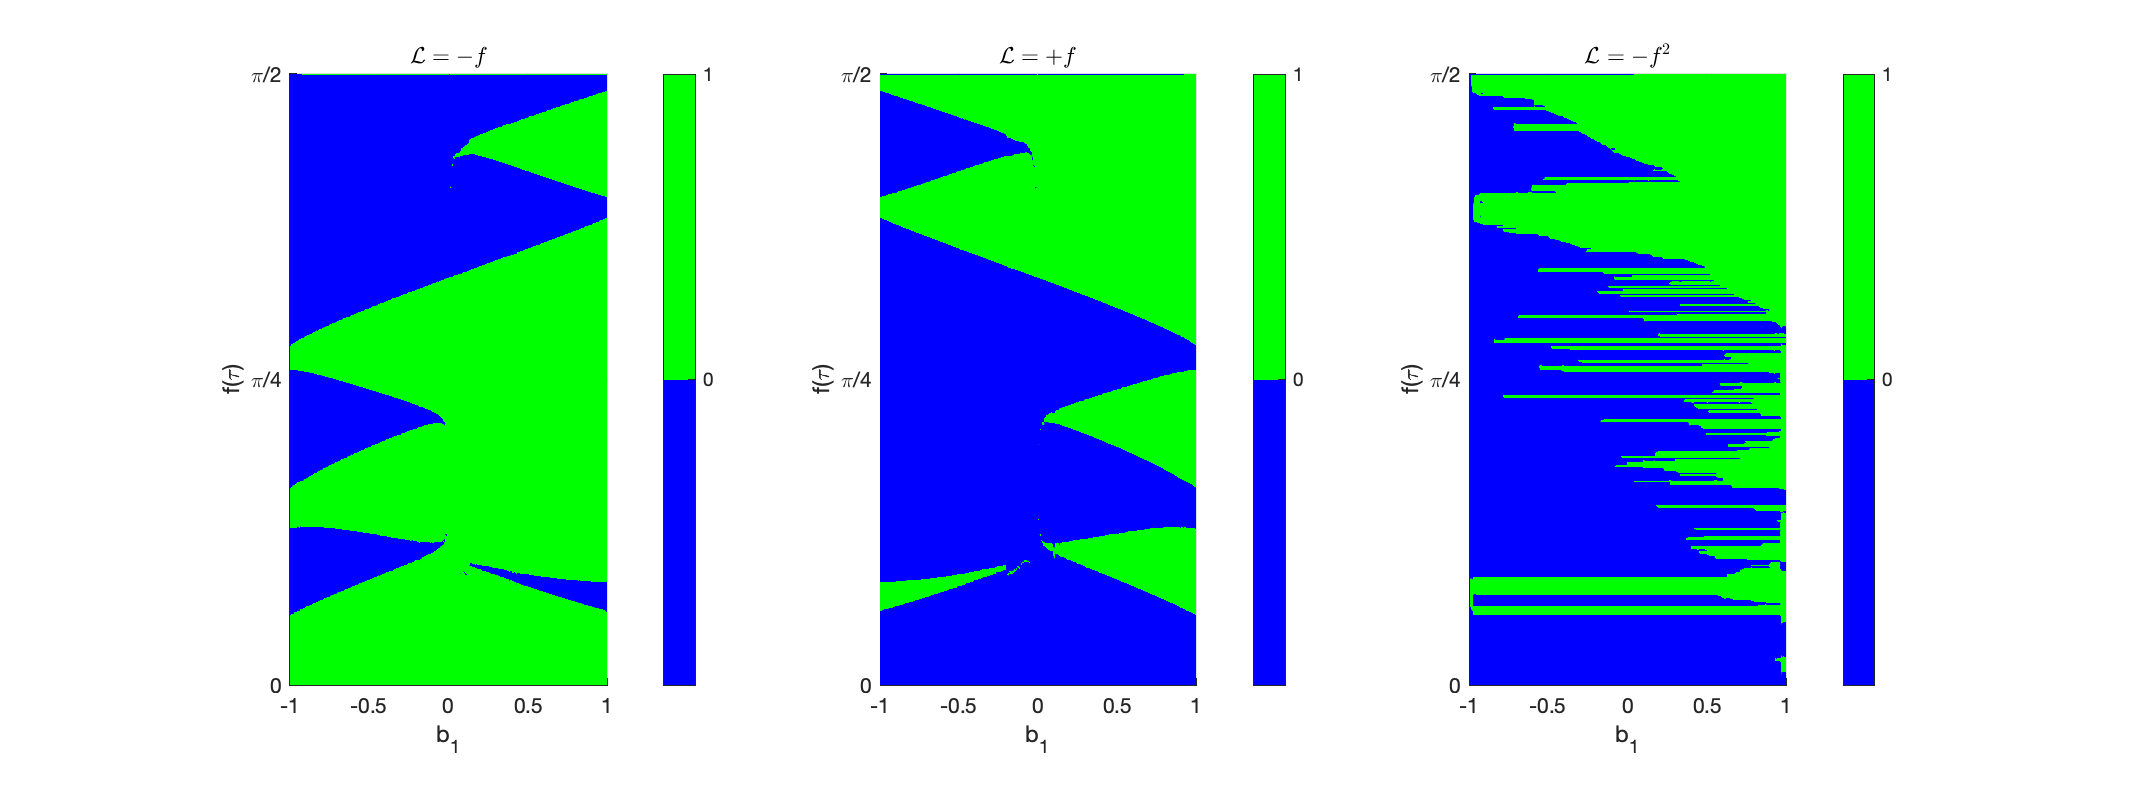
\includegraphics[scale=0.45]{img/EX01_surf_2LVL.eps}
            \caption{Comparison of solutions for different values of $m_a$. El problema con penalización $L(f) = -f$ y $L(f) = +f$ son equivalentes bajo una tranformación de inversión conrespecto a origen de coordendas y un cambio de signo.}
        \end{subfigure} 
        \hfill 
        \begin{subfigure}[b]{0.6\textwidth}
            \centering
            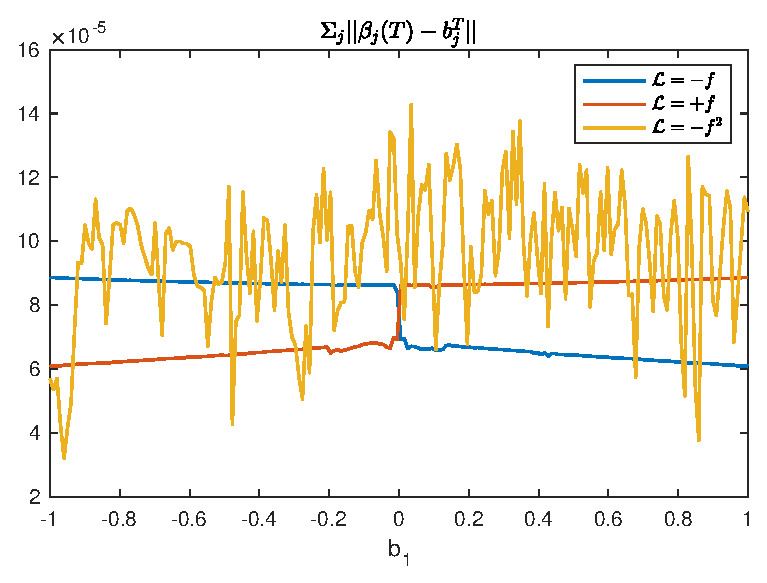
\includegraphics[scale=0.6]{img/EX01_2LVL.eps}
            \caption{Error}
        \end{subfigure}
        \caption{The order of magnitud of the distance of target}
        \label{ex01}
    \end{figure}


     
    \item \textbf{SHE para tres niveles}: Podemos ver que en el caso en el que el control $f(\tau)$ solo pueda tomar valores entre $[0,1]$ obtenemos señales que pueden tomar tres niveles en el intervalo $[0,2\pi]$ gracias a la simetría de cuarto de onda. Si resolvemos el problema de control óptimo pero esta vez cambiando las restricciones $|f(\tau)|<1$ por $\{0<f(\tau)<1\}$. Se ha realizado el mismo procedimiento que en el caso anterior, obteniendo soluciones para los mismo términos de penalización obteniendo la figura (\ref{ex3LVL}). Allí se muestra la continudad de las soluciones y que estas se encuentran en el orden de $10^{-4}$.
    



    \begin{figure}
        \centering
        \begin{subfigure}[b]{\textwidth}
            \centering
            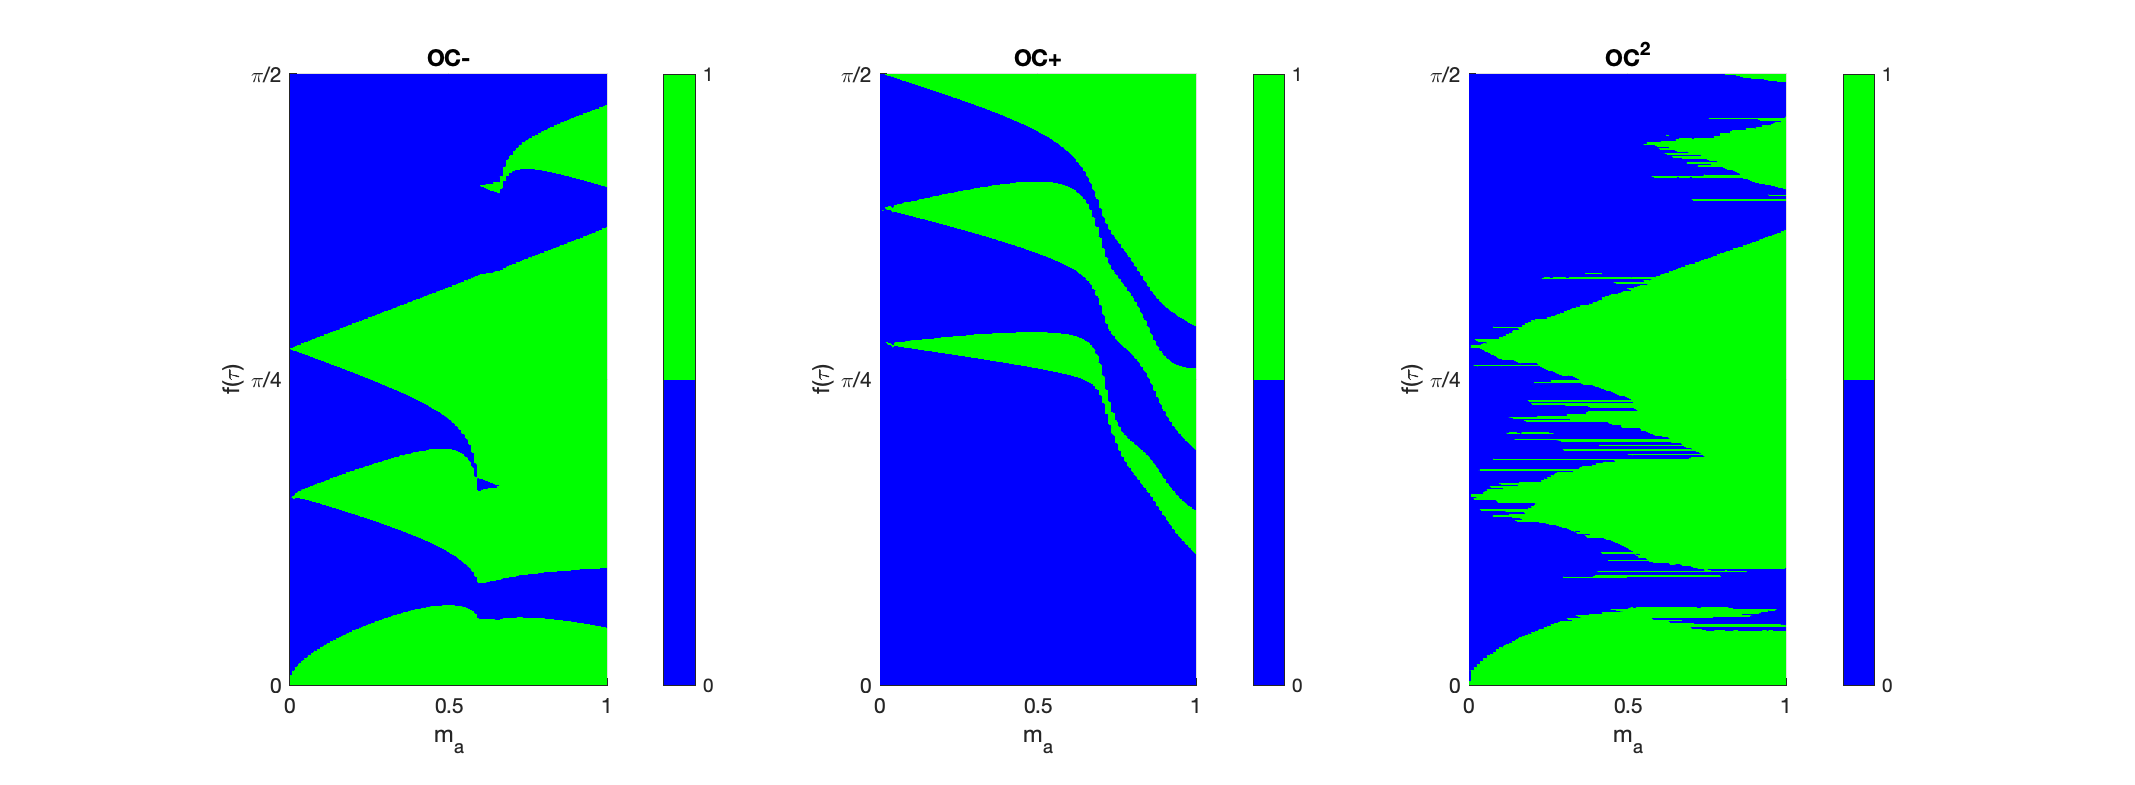
\includegraphics[scale=0.45]{img/EX01_surf_3LVL.eps}
            \caption{Soluciones para un control  con restriciones $0 \leq f\leq 1$ para obtener soluciones de tres niveles.}
        \end{subfigure} 
        \hfill \\
        \begin{subfigure}[b]{0.4\textwidth}
            \centering
            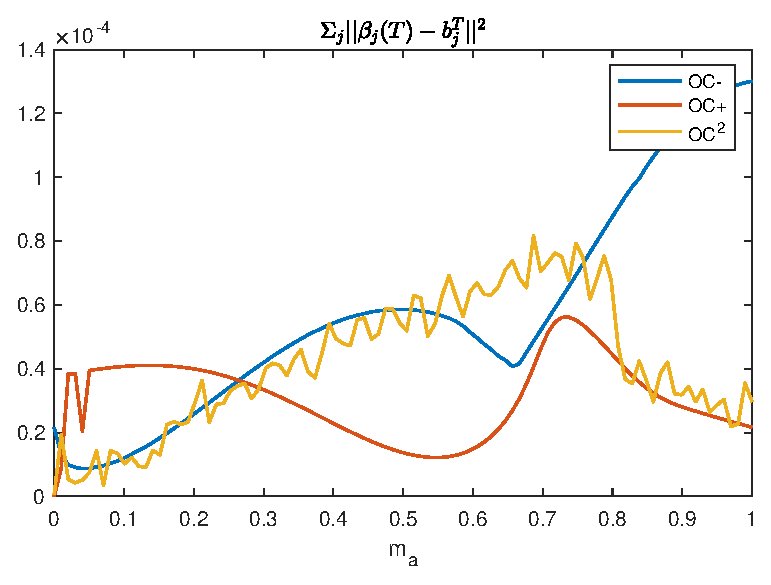
\includegraphics[scale=0.6]{img/EX01_3LVL.eps}
            \caption{error}
        \end{subfigure}
        \caption{Errors of solution in three level solutions}
        \label{ex3LVL}
    \end{figure}
    
    
    
      


    \item \textbf{Cambio en el número de conmunationes}: Gracias a la formulación de control óptimo para el problema SHE podemos variar el número de ángulos de conmuntación. 
    %
    Este es el cado del siguientes ejemplo, donde hemos tomado como conjunto de números pares $\mathcal{E}_b = \{1,3,9,13,17\}$,   además consideramos el vector objetivo $\bm{b}_T = [m_a,0,0,0,0]$, donde  $m_a \in [0,1]$ es un parámetro. 
    %
    En este problema hemos utilizado una penalización tipo $\mathcal{L} = f$ con un parémetro de penalización $\epsilon=10^{-4}$.
    %
    Podemos ver en la figura (\ref{disco}) como el problema de control óptimo es versátil y es capaz de mover entre varios conjuntos de soluciones.



    \begin{figure}[!ht]
        \centering
        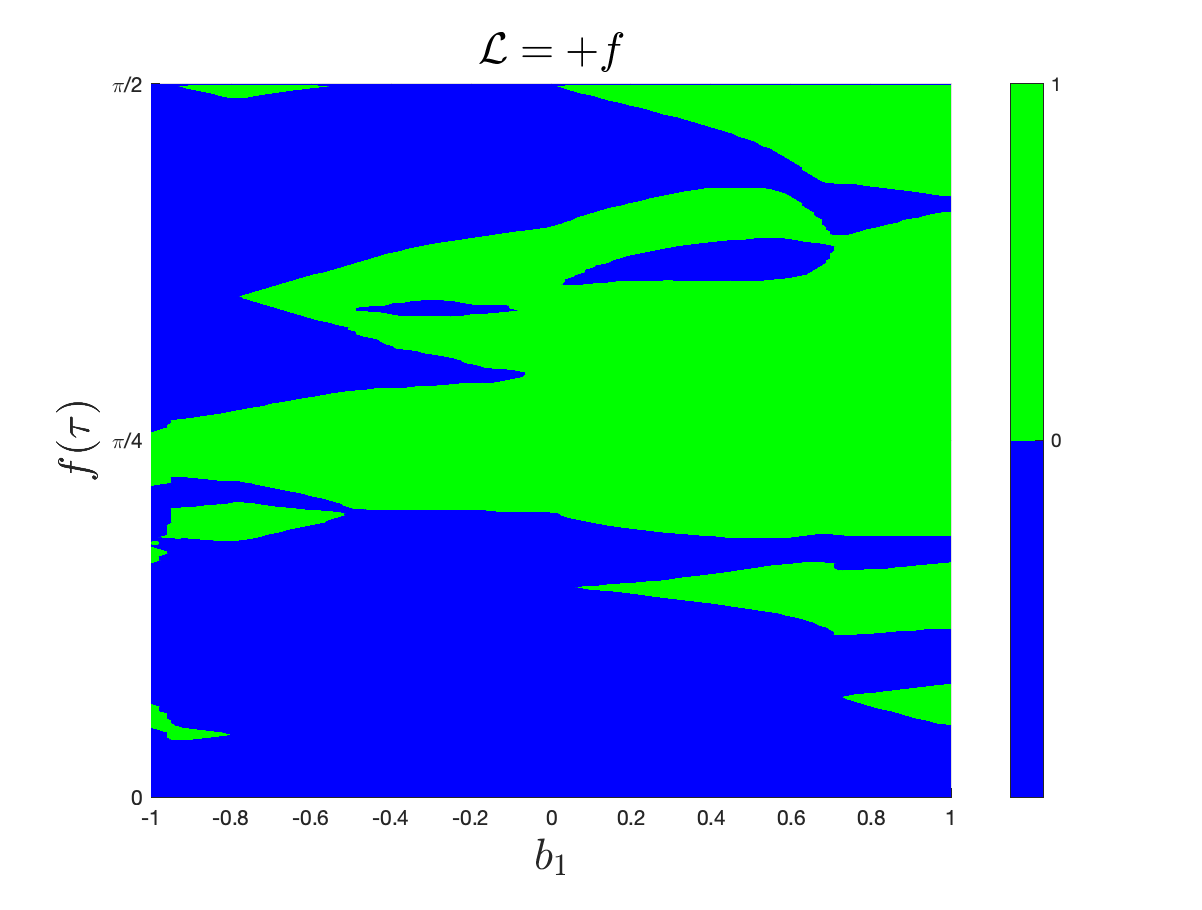
\includegraphics[scale=0.45]{img/EX00_surf_2LVL.eps}
        \caption{Discontinuidad en las soluciones obtenidas. Soluciones para SHE con simetría cuarto de onda con $\mathcal{E}_b = \{1,3,9,13,17\}$, donde $\bm{b}_T = [m_a,0,0,0,0]$ y  $m_a \in [0,1]$}
        \label{disco}
    \end{figure}


    
    \item \textbf{OCP para SHE con simetría de media onda}: Se ha relizado el caso de control óptimo de media onda con con $\mathcal{E}_a = \{1,3,5\}$ y  $\mathcal{E}_b = \{1,3,5,9\}$, donde $\bm{a}_T = [m_a,0,0]$, $\bm{b}_T = [m_a,m_a,0,0]$ y  $m_a \in [-0.6,0.6]$. Se ha elegido la penalización $L(f) = +f$
    \begin{figure}
        \centering
        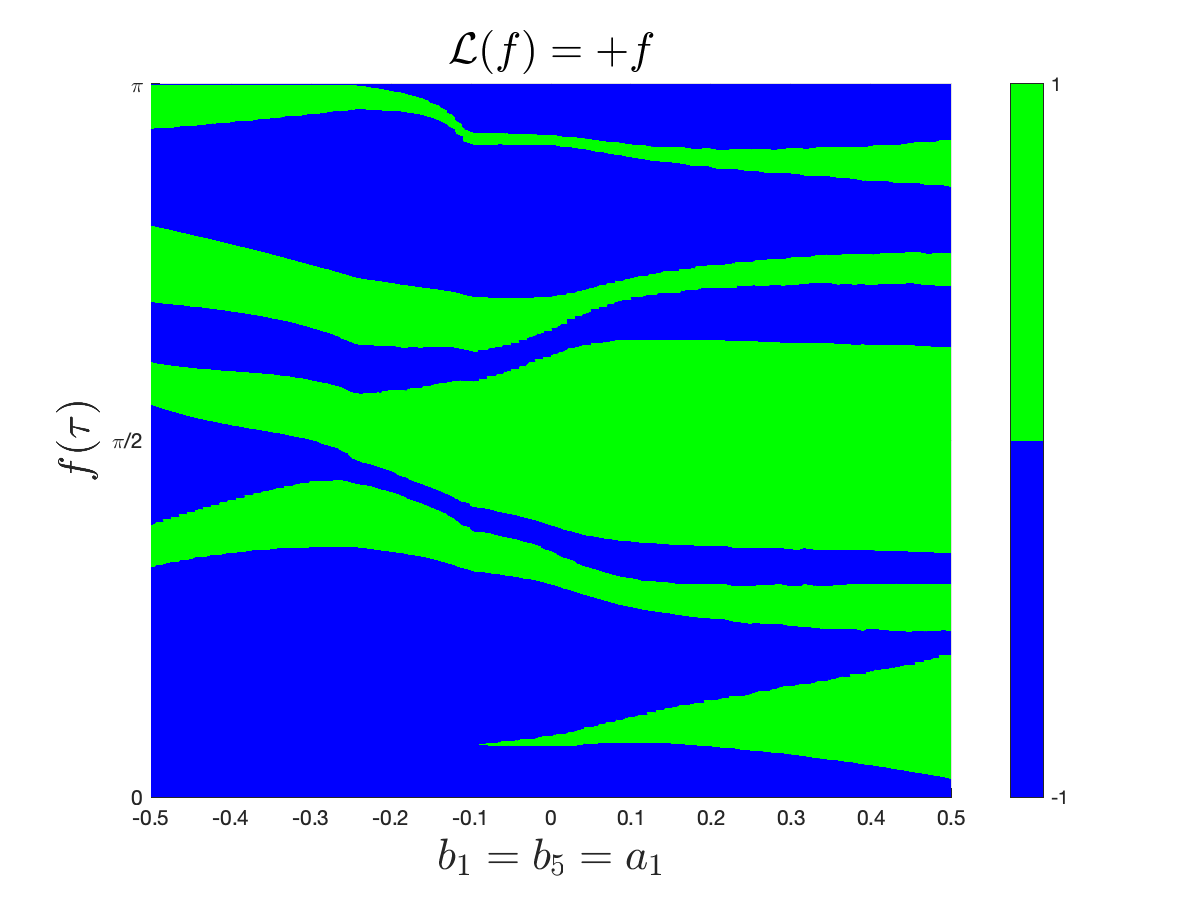
\includegraphics[scale=0.45]{img/alphabeta.eps}
        \caption{Discontinuidad en las soluciones obtenidas. Soluciones para SHE con simetría media de onda con $\mathcal{E}_a = \{1,3,5\}$ y  $\mathcal{E}_b = \{1,3,5,9\}$, donde $\bm{a}_T = [m_a,0,0]$, $\bm{b}_T = [m_a,m_a,0,0]$ y  $m_a \in [-0.6,0.6]$}. 

    \end{figure}





    \begin{figure}
        \centering
        \begin{subfigure}[b]{\textwidth}
            \centering
            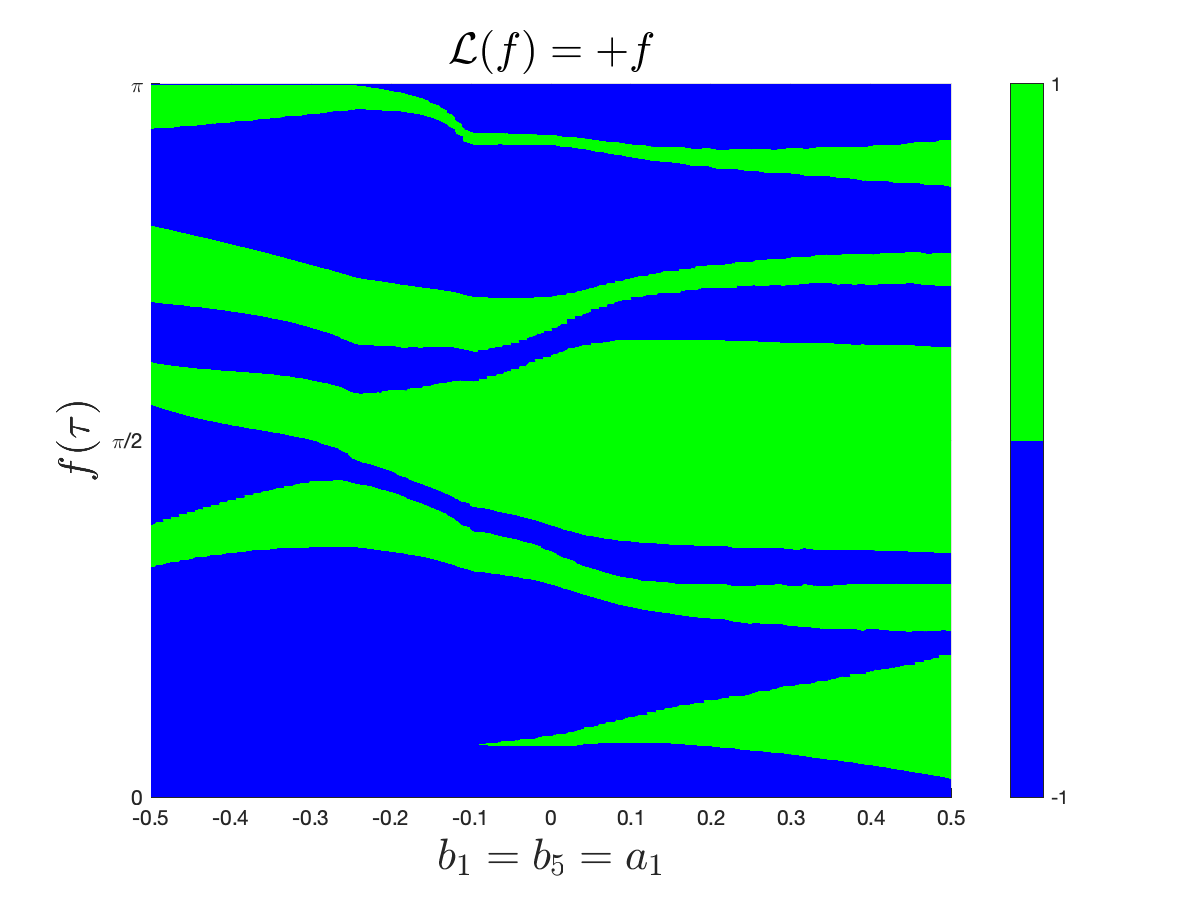
\includegraphics[scale=0.4]{img/alphabeta.eps}
            \caption{Discontinuidad en las soluciones obtenidas. Soluciones para SHE con simetría media de onda con $\mathcal{E}_a = \{1,3,5\}$ y  $\mathcal{E}_b = \{1,3,5,9\}$, donde $\bm{a}_T = [m_a,0,0]$, $\bm{b}_T = [m_a,m_a,0,0]$ y  $m_a \in [0,1]$}
        \end{subfigure} 
        \hfill 
        \begin{subfigure}[b]{\textwidth}
            \centering
            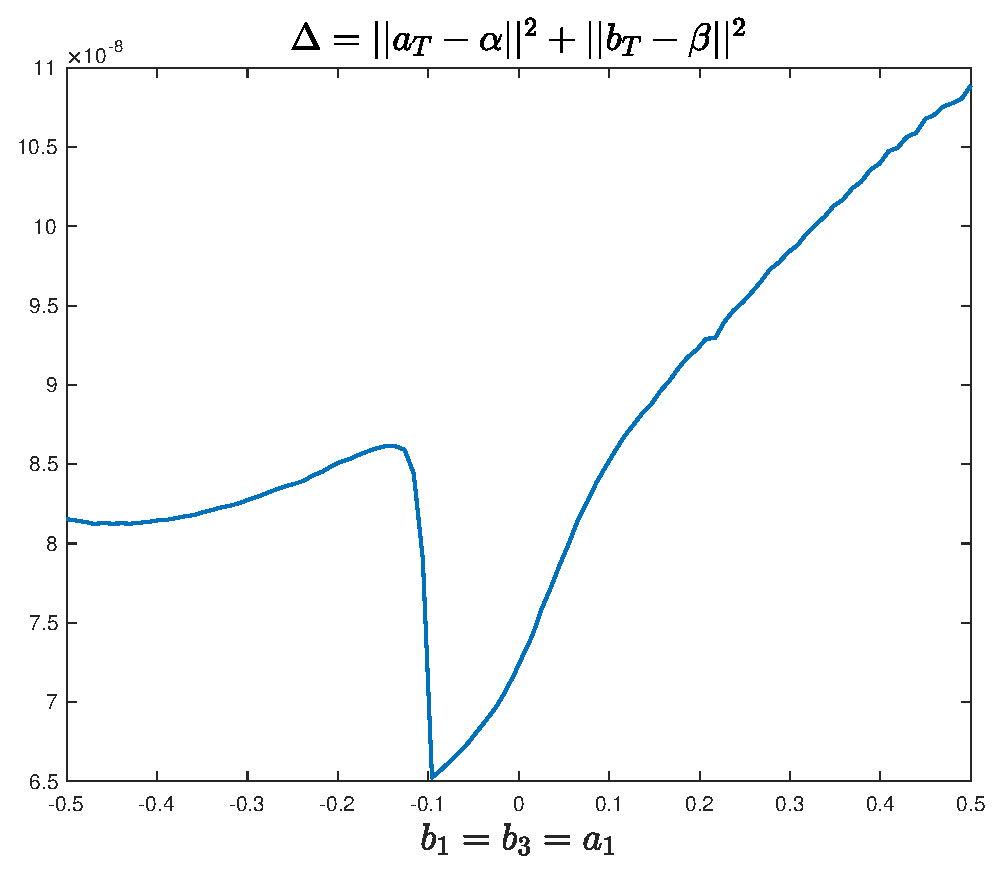
\includegraphics[scale=0.4]{img/alphabeta_error.eps}
            \caption{error}
        \end{subfigure}
        \caption{Errors of solution in three level solutions}
        \label{ex3LVL}
    \end{figure}


\end{enumerate}






